%----------------------------------------------------------------------------------------------------------------------

\begin{frame}[<+-| alert@+>]{Haven't researchers tried using Features before?}

\begin{itemize}[noitemsep,label=\textbullet,topsep=2pt,parsep=2pt,partopsep=2pt]
\item The idea is not completely new. At very basic/singular feature level, but not for full set of features, or for building a reasonably complex part. And not for Sheet Metal features.

%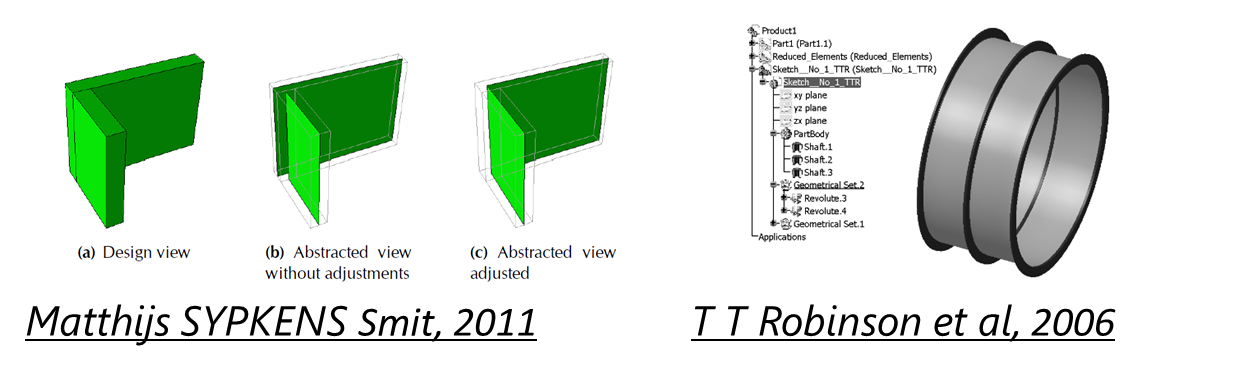
\includegraphics[scale=0.35]{../Common/images/TriedBefore.png}

\item Decomposition is used to get feature tree like (or CSG like) representation first, then the simpler primitives are used to create midsurfaces \cite{Chong2004}
\item Researchers probably could not get handle on the internal feature information as it was hidden for many years for proprietary reasons. 

\item But, this feature information was readily available for internal folks to develop algorithms upon. Then why have Companies not used this approach so far?

\end{itemize}
\end{frame}
%----------------------------------------------------------------------------------------------------------------------

\begin{frame}[<+-| alert@+>]{Why Companies did not leverage the feature information?}

\begin{itemize}[noitemsep,label=\textbullet,topsep=2pt,parsep=2pt,partopsep=2pt]
\item CAD and CAE fields had their own way, separately for a long time. Integrating these domains has not happened fully yet. So, even now, data is transferred between them via neutral file formats. So CAE gets to see final shape only and not how part is made.
\item Some Solid Modelers allow only Manifold modeling, say Unigraphics, for most of the time, works under Manifold flag of Parasolid Kernel
\item  Some modelers DO support Non-Manifold like ACIS, CATIA, Inventor, Pro/E. These established Solid modelers would find it risky to embed non-manifold data model (surfaces) in existing Manifold data model, as they would have to alter most of the existing functionality to react to this addition. It would be highly impractical to change their core modeling data structures and paradigm now, to cater only to some specialized down-stream applications like CAE.


\end{itemize}
\end{frame}
%----------------------------------------------------------------------------------------------------------------------

\begin{frame}[<+-| alert@+>]{What's meant by 'better' Midsurface?}
\begin{itemize}[noitemsep,label=\textbullet,topsep=2pt,parsep=2pt,partopsep=2pt]
\item As Midsurfaces are generated Face-Pair wise, they need to be then stitched together to form a continuous shape. Connected  disjoint midsurfaces by extend-trim depends on individual surface-shapes, estimation of extension etc. Midsurface is expected to have proper connectivity  (no gaps) between individual patches and it should follow shape of the base part.
\item {\it A geometric similarity evaluation technique based on the Hausdorff distance and secondly a topological similarity evaluation method which uses geometry graph attributes as the basis for comparison} \cite{Lockett2008}
\end{itemize}
\end{frame}
%----------------------------------------------------------------------------------------------------------------------

\begin{frame}{When-What}
\begin{itemize}[noitemsep,label=\textbullet,topsep=2pt,parsep=2pt,partopsep=2pt]
\item \textbf{1967} Blum: MAT
\item \textbf{1994} Dabke: Features for Idealization
\item \textbf{1996} Armstrong: MAT for CAE
\item \textbf{1996} Rezayat: MA SDRC
\item \textbf{1999} Fischer: Parametric Midcurves
\item \textbf{2002} Deng: FBD Simplification
\item \textbf{2005} Stolt: Pocket Pad based Midsurface
\item \textbf{2007} Robinson: Sketch based Midsurface
\item \textbf{2012} Russ: FBD defeaturing
\item \textbf{2013} Woo: Decomp, per feature Midsurface
\end{itemize}

%Notes: 

\end{frame}


%----------------------------------------------------------------------------------------------------------------------

\begin{frame}[<+-| alert@+>]{T Robinson, C Armstrong. Univ of Belfast, UK \cite{Robinson2007}}

\begin{columns}[T]

\column{0.6\textwidth}
	%\vspace{-3cm}
	\begin{itemize}[noitemsep,label=\textbullet,topsep=2pt,parsep=2pt,partopsep=2pt]
	\item Automated mixed-dimensional model from CAD for aerospace structures.
	\item Utilizes information in CAD feature tree to locate sketches and then features built on top of it like Sweep, Revolve.
	\item Limited feature-set, no feature interaction which is a key problem
	\end{itemize}
\column{0.4\textwidth}
	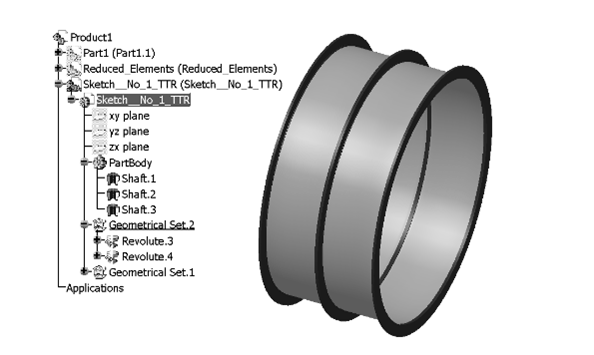
\includegraphics[scale=0.5]{../Common/images/Robinson.png}
\end{columns}

%Notes: 
\end{frame}

%----------------------------------------------------------------------------------------------------------------------

\begin{frame}[<+-| alert@+>]{S H Lee, D P Sheen. Korea  \cite{Sheen2008}}


\begin{itemize}[noitemsep,label=\textbullet,topsep=2pt,parsep=2pt,partopsep=2pt]
	\item Solid Deflection: Solid is assumed to be created by inflating air. So deflating would create zero-thickness Midsurface model.
	\item Involves Face-pair detection and face geometry replacement. Topology is kept intact.
Bigger of the two is offset-ed. 
	\item Tolerance is increased so as to make them look like connected but they are not.
	\item Does not talk about any non-trivial face-pair interactions and Booleans

	\end{itemize}

	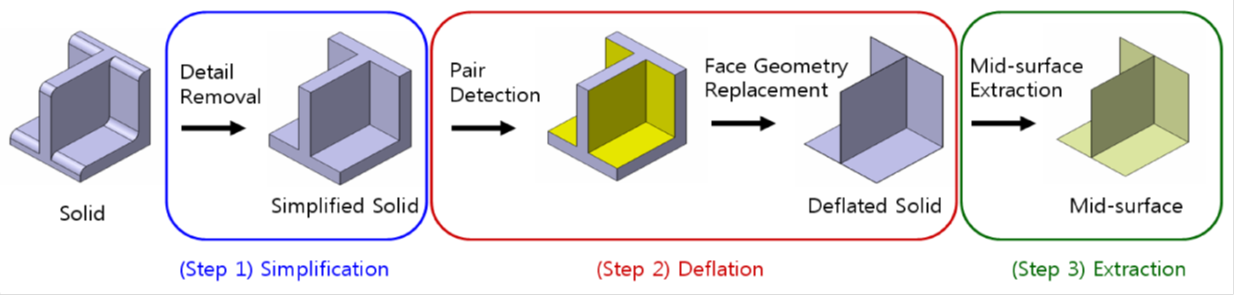
\includegraphics[scale=0.4]{../Common/images/Sheen.png}

%Notes: 
\end{frame}

%----------------------------------------------------------------------------------------------------------------------

\begin{frame}[<+-| alert@+>]{Helen Lockett, Cranfield, UK \cite{Lockett2008}}

\begin{columns}[T]

\column{0.5\textwidth}

	\begin{itemize}[noitemsep,label=\textbullet,topsep=2pt,parsep=2pt,partopsep=2pt]
	\item Used Midsurfaces as Feature recognizer in Injection Molding domain
	\item Found measures to assess quality of midsurfaces
	\item Geometric Similarity: Hausdorff distance (maximum dissimilarity between two similar shapes)
	\item Topological Similarity:  based on number of Midsurface edges wrt corresponding edges in the Solid
	\end{itemize}

\column{0.5\textwidth}
	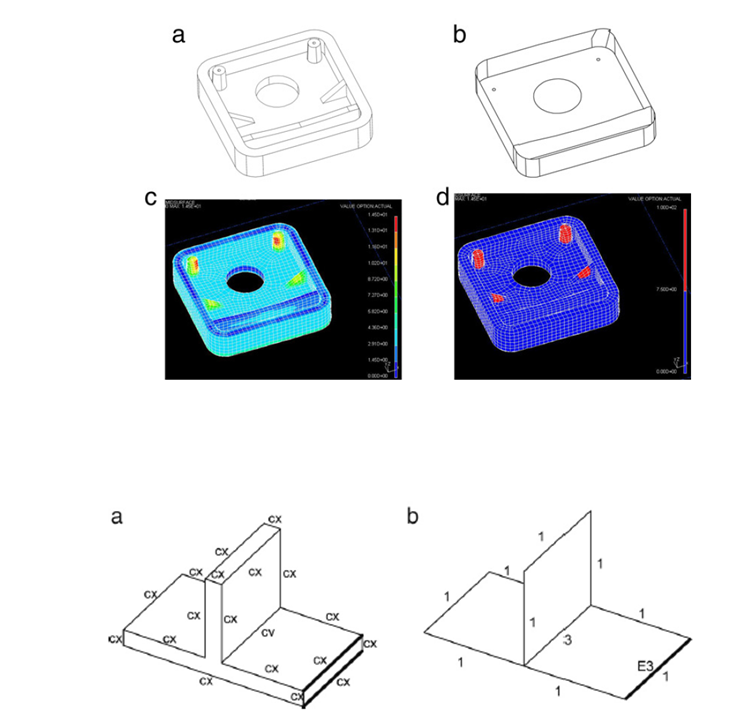
\includegraphics[scale=0.4]{../Common/images/Lockett.png}
\end{columns}

%Notes: 
\end{frame}
%----------------------------------------------------------------------------------------------------------------------

\begin{frame}[<+-| alert@+>]{Others}

\begin{columns}[T]

\column{0.75\linewidth}
	%\vspace{-5cm}

	\begin{itemize}[noitemsep,label=\textbullet,topsep=2pt,parsep=2pt,partopsep=2pt]
	\item Chong, NUS, Singapore, 2004 \cite{Chong2004}:

		\begin{itemize}[noitemsep,label=\textbullet,topsep=2pt,parsep=2pt,partopsep=2pt]
		\item Model is decomposed into simpler solids
		\item Solids extract their own midsurfaces
		\item Focuses more on extracting/decomposing  
		\end{itemize}

	\item Brian Russ, MS, Univ of Maryland, 2012 \cite{Russ2012}: 
		\begin{itemize}[noitemsep,label=\textbullet,topsep=2pt,parsep=2pt,partopsep=2pt]
		\item Feature based Model simplification.
		\item Rule based approach Fillet/Hole suppression
		\end{itemize}

	\item M S Smit, PhD, TU Delft, 2011 \cite{Smit2011}:
		\begin{itemize}[noitemsep,label=\textbullet,topsep=2pt,parsep=2pt,partopsep=2pt]
		\item Feature based re-meshing
		\item Bidirectional update
		\item Clearly expresses need for research
		\end{itemize}
	\end{itemize}

\column{0.25\linewidth}
	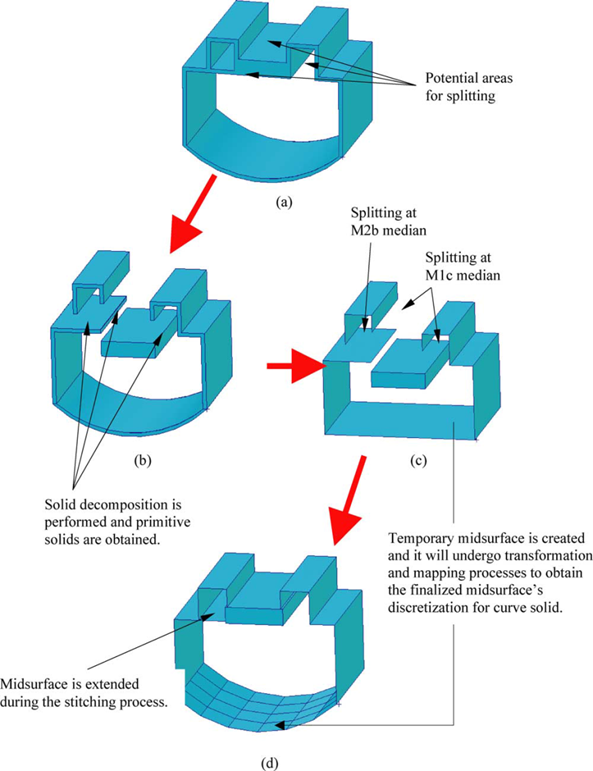
\includegraphics[width=0.9\linewidth]{../Common/images/Chong.png}
\end{columns}

%Notes: 
\end{frame}
%----------------------------------------------------------------------------------------------------------------------

\begin{frame}[<+-| alert@+>]{Literature Survey - Conclusions}
\begin{itemize}[noitemsep,label=\textbullet,topsep=2pt,parsep=2pt,partopsep=2pt]

\item Model Simplification is essential even when computation power has increased dramatically, because:
\begin{itemize}[noitemsep,label=\textbullet,topsep=2pt,parsep=2pt,partopsep=2pt]
\item more complex problems can be solved
\item more design iterations can be performed
\end{itemize}

\item Which Domain?
\begin{itemize}[noitemsep,label=\textbullet,topsep=2pt,parsep=2pt,partopsep=2pt]
\item Injection Molding parts are most complex due to draft and have most demand 
\item Sheet Metal parts are relatively easy, create surfaces but fail in connections. 
\end{itemize}

\item Why Mid and not just one side?
\begin{itemize}[noitemsep,label=\textbullet,topsep=2pt,parsep=2pt,partopsep=2pt]
\item Geometrical issues: - sides do not connect well, 
\item Analysis issues:- It does not matter for ultra thin parts but for normal thin parts ($L/t > 100$ and $< 750$), Midsurface is essential
\end{itemize}

\end{itemize}

%Notes: 

\end{frame}


%----------------------------------------------------------------------------------------------------------------------
\begin{frame}[<+-| alert@+>]{Literature Survey - Conclusions}
\begin{itemize}[noitemsep,label=\textbullet,topsep=2pt,parsep=2pt,partopsep=2pt]

\item Medial generation method?
\begin{itemize}[noitemsep,label=\textbullet,topsep=2pt,parsep=2pt,partopsep=2pt]
\item MAT: unsuitable as it creates branches
\item MA: Face pairing is complex
\item Feature based: So far Sweep based and primitives have been tried. No one, so far has worked on feature interactions, extend-trim and non-manifold boolean to get connected Midsurface
\end{itemize}

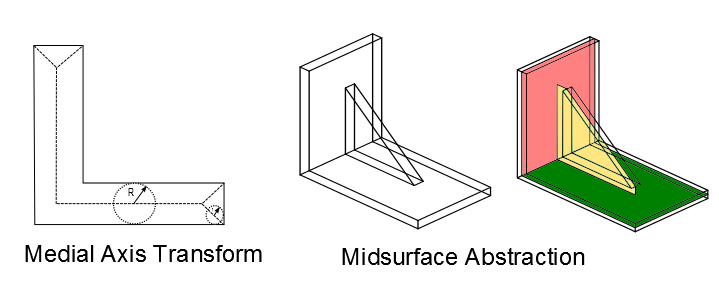
\includegraphics[scale=0.4]{../Common/images/MAT_Midsurf.png}

\end{itemize}

%Notes: 

\end{frame}


%----------------------------------------------------------------------------------------------------------------------
\begin{frame}[<+-| alert@+>]{Literature Survey - Conclusions}
\begin{itemize}[noitemsep,label=\textbullet,topsep=2pt,parsep=2pt,partopsep=2pt]

\item ``There is a definite need for a dimensional reduction capability that is more powerful and easier to use than those currently available in the market. Such a capability should deliver an automated scheme for handling cases that have traditionally caused problems for algorithms in this field'' - \cite{Stanley2010}

\item ``Much of research is yet to be done, use of symmetry, various features, various abstractions are not yet handled.''- \cite{Smit2011}

%\vspace{1cm}

%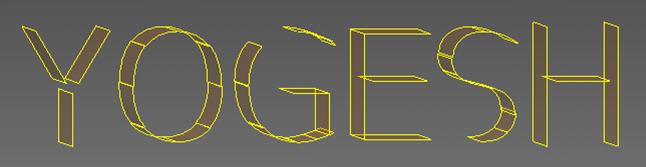
\includegraphics[scale=0.4]{../Common/images/YOGESH_Midsurf.png}


\end{itemize}

\def \myfigcommcolumnwidth{0.28}

\begin{figure}[h!]
\centering     %%% not \center
\subfloat[Model]{\label{fig_mmodel}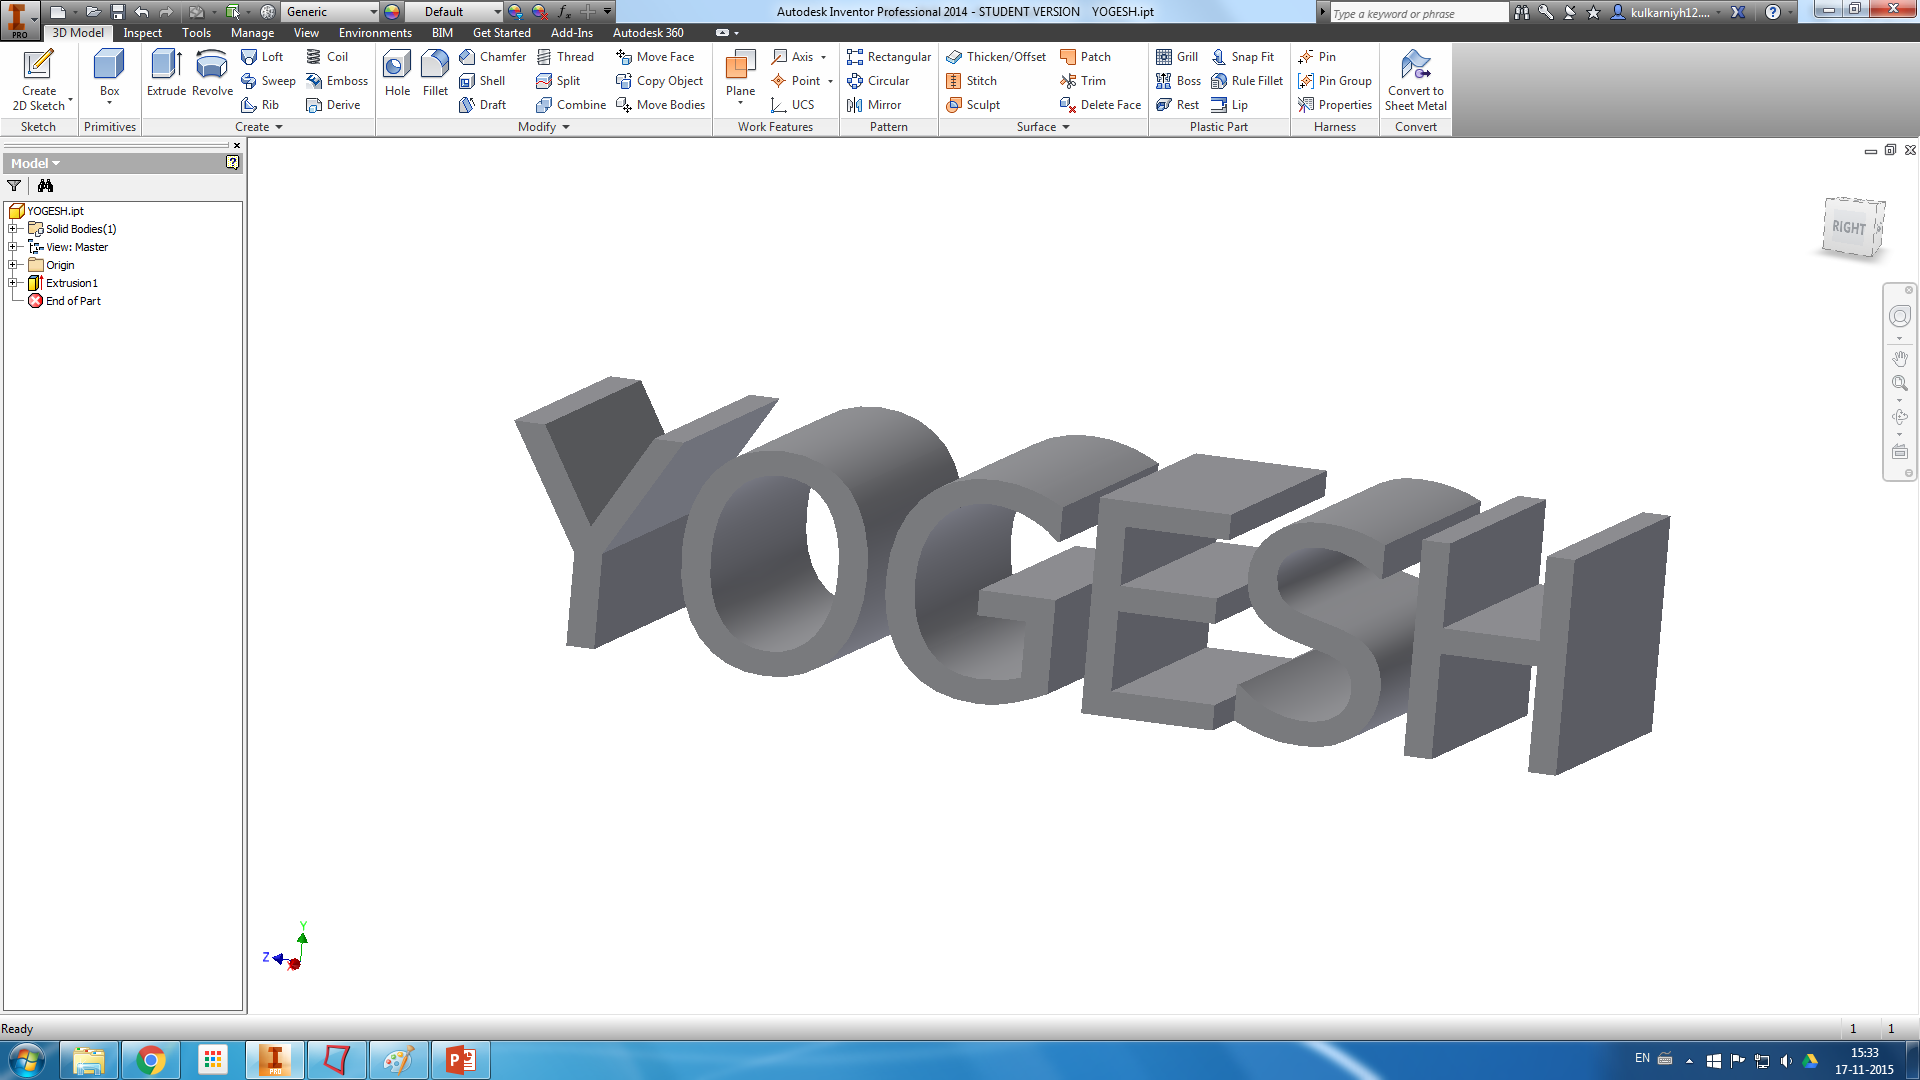
\includegraphics[width=\myfigcommcolumnwidth\linewidth]{../Common/images/Yogesh_Inv}} \quad
\subfloat[Midsurface: Application 1]{\label{fig_mcad}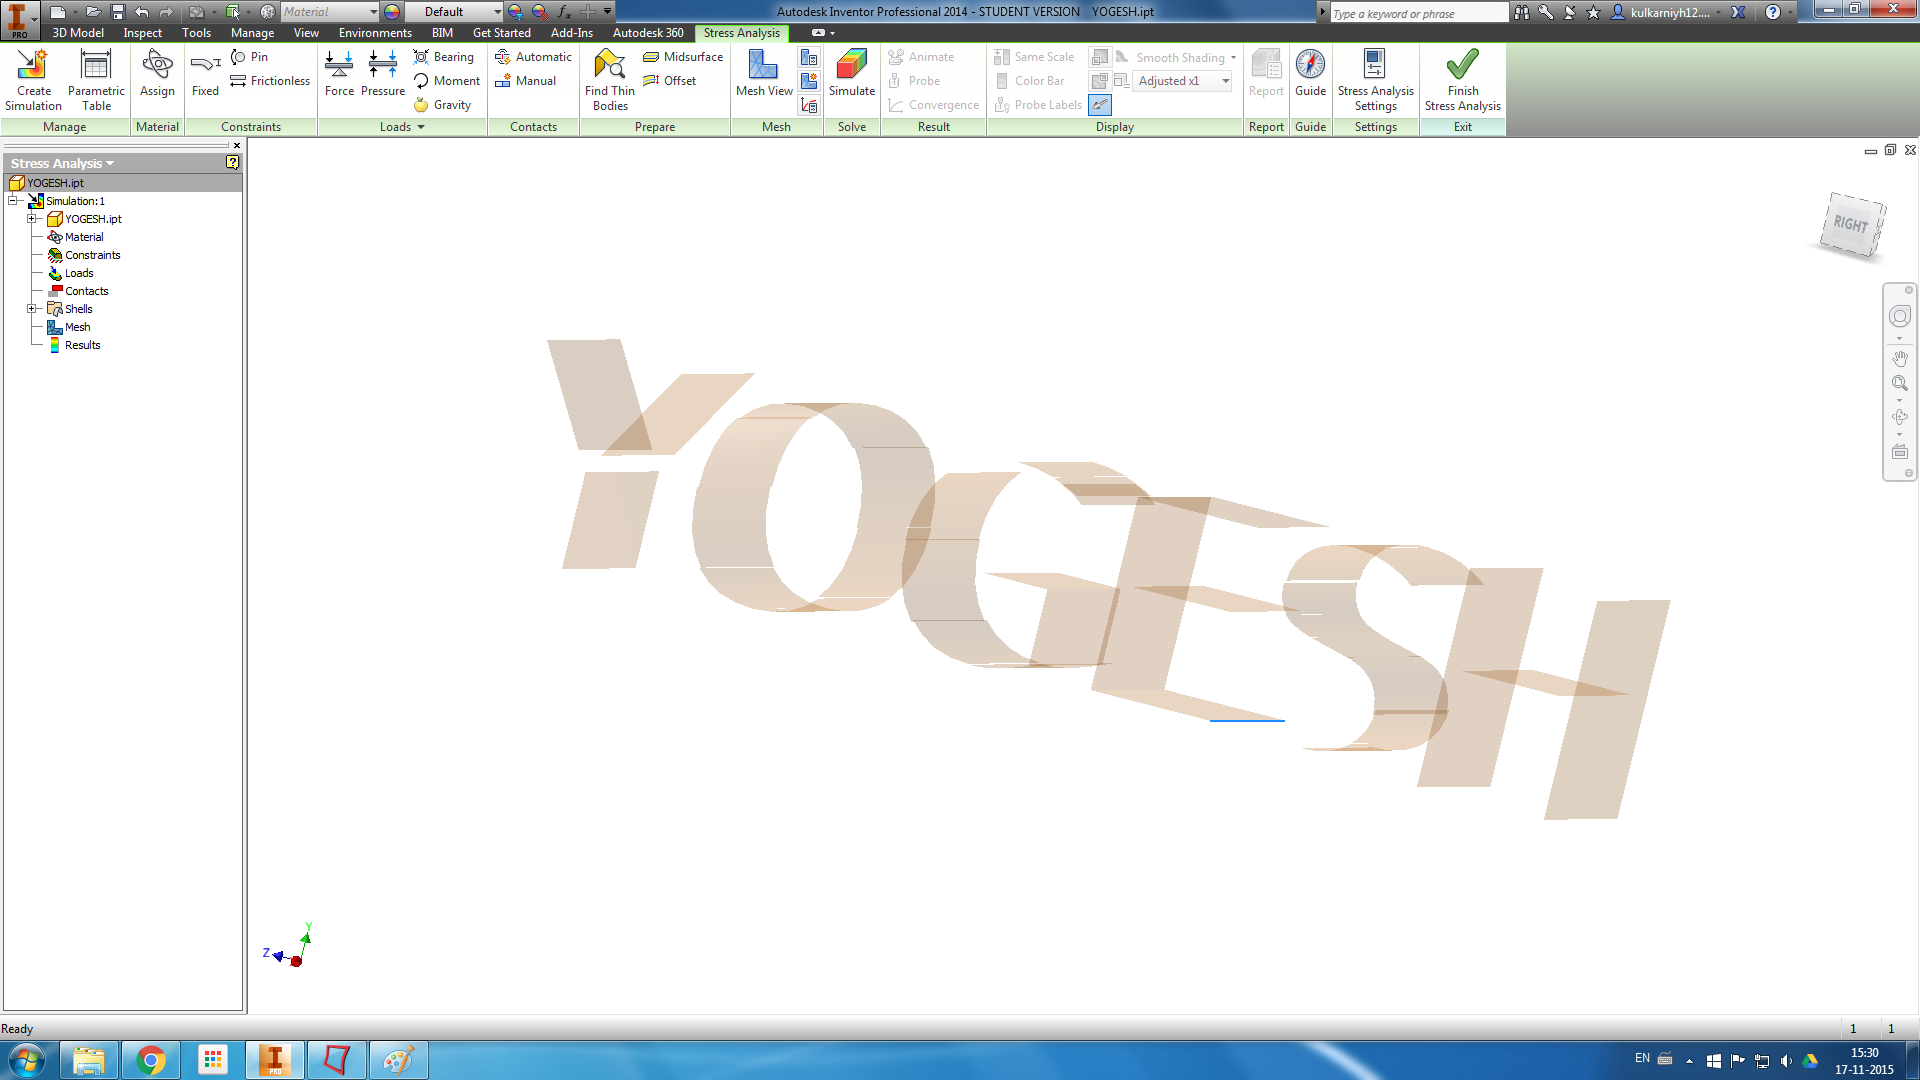
\includegraphics[width=\myfigcommcolumnwidth\linewidth]{../Common/images/Yogesh_InvMids}} \quad
\subfloat[Midsurface: Application 2]{\label{fig_mcae}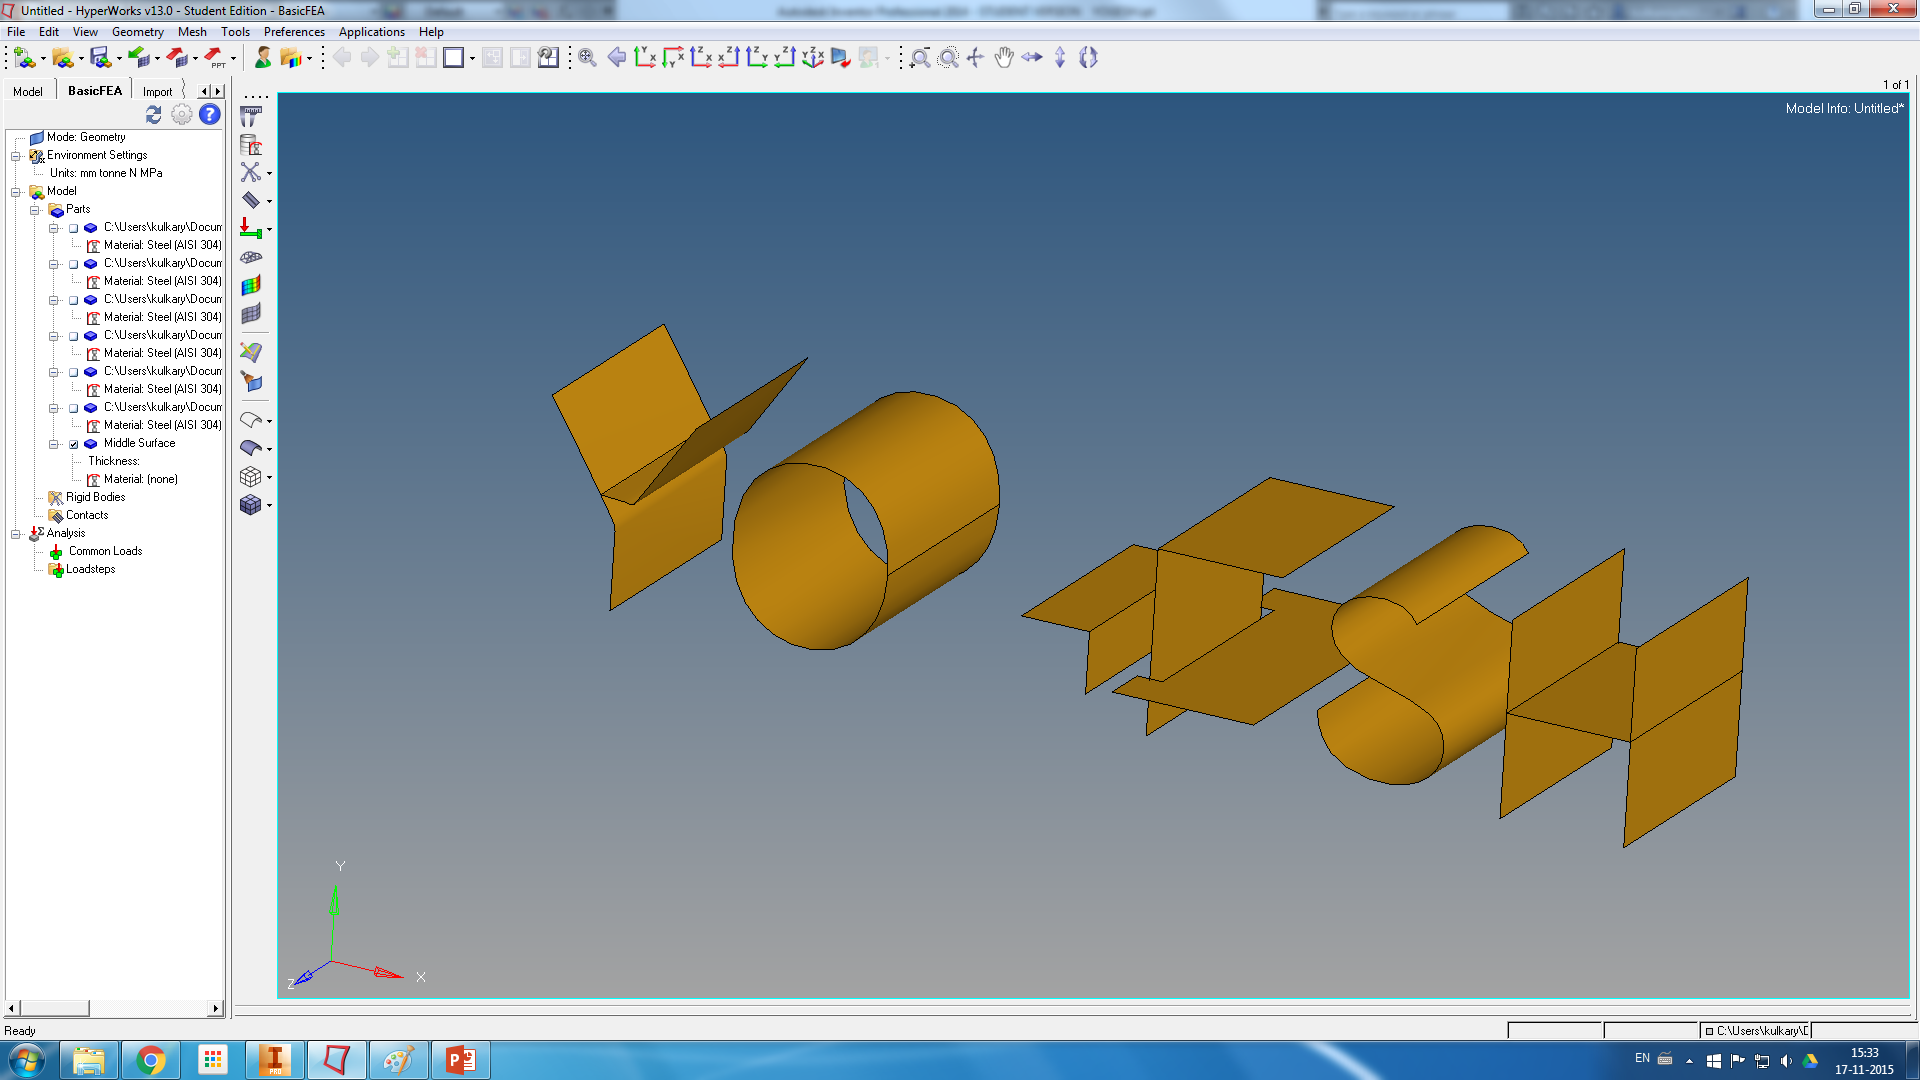
\includegraphics[width=\myfigcommcolumnwidth\linewidth]{../Common/images/Yogesh_HM_notOK}} 
\caption{Midsurface outputs of commercial applications}
  \label{fig_comm}
\end{figure}
%Notes: 

\end{frame}

%----------------------------------------------------------------------------------------------------------------------
\begin{frame}[<+-| alert@+>]{Literature Survey - Conclusions}

\centering
{\em \bfseries \large Thus, so far, there has been a limited success in the objective of computing a well-connected midsurface. This work plans to leverage feature information to achieve this objective.}


%Notes: 

\end{frame}
